\subsection{Делимость и факториальные кольца}

\textbf{До конца раздела} зафиксируем область целостности $K$.

\begin{definition}
	Пусть $a, b \in K$. Говорят, что \textit{$a$ делит $b$}, или \textit{$b$ делится на $a$}, если $\exists c \in K: b = ac$. Обозначение "--- $a \mid b$.
\end{definition}

\begin{note}
	Отношение делимости является отношением предпорядка, но не является отношением порядка, поскольку для него не выполнена антисимметричность: если $a \mid b$ и $b \mid a$, то $b = ac$ и $a = bd$, $c, d \in K$, причем $cd = 1$, то есть $c, d \in K^*$.
\end{note}

\begin{definition}
	Группа $K^*$ действует на $K$ умножениями. Орбиты этого действия называются \textit{классами ассоциированности}. Элементы $a, b \in K$ называются \textit{ассоциированными}, если они лежат в одном классе ассоциированности, то есть $\exists c \in K^*: a = bc$. Обозначение "--- $a \sim b$.
\end{definition}

\begin{proposition}
	Отношение ассоциированности является отношением эквивалентности на $K$.
\end{proposition}

\begin{proof}
	Отношение ассоциированности совпадает с отношением эквивалентности относительно действия $K^*$ на $K$ умножениями.
\end{proof}

\begin{proposition}
	Пусть $a, b \in K$. Тогда эквивалентны следующие утверждения:
	\begin{enumerate}
		\item $a \sim b$
		\item $\{c \in K: a \mid c\} = \{c \in K: b \mid c\}$
		\item $\{c \in K: c \mid a\} = \{c \in K: c \mid b\}$
	\end{enumerate}
\end{proposition}

\begin{proof} Докажем, что $1 \lra 2$, поскольку эквивалентность $1 \lra 3$ доказывается аналогично:
	\begin{itemize}
		\item[$\ra$] Если $a = bd$, $d \in K^*$, то, в силу обратимости элемента $d$, $a \mid c \lra \exists \alpha \in K: c = a\alpha \hm\lra \exists \alpha \in K: c = bd\alpha \hm\lra \exists \beta \in K: c = b\beta \lra b \mid c$.
		\item[$\la$] Из условия следует, что $a \mid b$ и $b \mid a$, поэтому $a \sim b$.\qedhere
	\end{itemize}
\end{proof}

\begin{definition}
	\textit{Расширение кольца $\Z$ числом $\alpha \in \Cm$} "--- это наименьшее по включению подкольцо в $\Cm$, содержащее $\Z$ и $\alpha$. Обозначение "--- $\Z[\alpha]$.
\end{definition}

\begin{proposition}
	$\forall \alpha \in \Cm: \Z[\alpha] = \{p(\alpha): p \in \Z[x]\}$.
\end{proposition}

\begin{proof}
	Обозначим множество справа через $S$. С одной стороны, очевидно, что $S \subset \Z[\alpha]$. С другой стороны, $S$ "--- кольцо, поскольку оно замкнуто относительно сложения и умножения, поэтому $\Z[\alpha] \subset S$.
\end{proof}

\begin{example}
	Рассмотрим $\Z[i] = \{a + bi: a, b \in \Z\}$ "--- \textit{гауссовы числа}. Покажем, что $\Z[i]^* \hm= \{\pm1, \pm i\}$. Для этого определим на $\Z[i]$ \textit{норму} $N : \Z[i] \to \N \cup \{0\}$ следующим образом: для всех $a + bi \in \Z[i]$ положим $N(a + bi) := a^2 + b^2$. Заметим, что тогда для всех $z, w \in \Z[i]$ выполнено $N(zw) = N(z)N(w)$. Значит, все обратимые элементы в $\Z[i]$ имеют норму, равную единице, тогда непосредственной проверкой получим, что $\Z[i]^* = \{\pm1, \pm i\}$.
	
	\pagebreak
	На комплексной плоскости гауссовы числа образуют решетку следующего вида (синим отмечено $\Z[i]^*$, красным "--- пример четверки ассоциированных элементов):
	\begin{center}
		\scalebox{0.85}{
		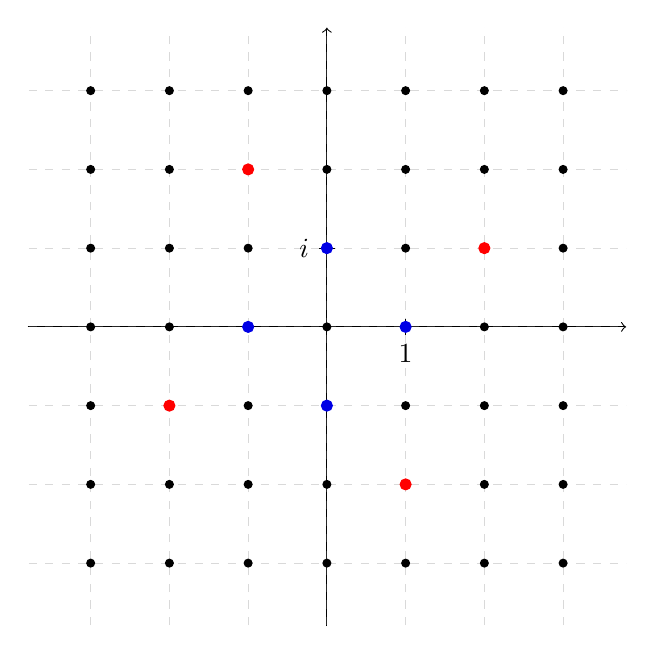
\begin{tikzpicture}
			\clip (-3.8, -3.8) rectangle (3.8, 3.8);
			\draw [->] (-3.8, 0) -- (3.8, 0);
			\draw [->] (0, -3.8) -- (0, 3.8);
			\draw[style=help lines,dashed, thin, gray, opacity=0.3] (-4,-4) grid (4,4);
			
			\draw (1,3pt) -- (1,-3pt) node [below] {$1$};
			\draw (3pt,1) -- (-3pt,1) node [left] {$i$};
			
			\foreach \x in {-5, -4, ..., 5}{
				\foreach \y in {-5, -4, ..., 5}{
					\node[draw,circle,inner sep=1pt,fill] at (\x, \y) {};
				}
			}
		
			\node[draw,circle,inner sep=1.4pt,fill,black!10!blue] at (0, 1) {};
			\node[draw,circle,inner sep=1.4pt,fill,black!10!blue] at (1, 0) {};
			\node[draw,circle,inner sep=1.4pt,fill,black!10!blue] at (0, -1) {};
			\node[draw,circle,inner sep=1.4pt,fill,black!10!blue] at (-1, 0) {};
			
			
			\node[draw,circle,inner sep=1.4pt,fill,red] at (2, 1) {};
			\node[draw,circle,inner sep=1.4pt,fill,red] at (1, -2) {};
			\node[draw,circle,inner sep=1.4pt,fill,red] at (-2, -1) {};
			\node[draw,circle,inner sep=1.4pt,fill,red] at (-1, 2) {};
		\end{tikzpicture}
		}
	\end{center}
\end{example}

\begin{example}
	Рассмотрим $\Z[\omega] = \{a + b\omega: a, b \in \Z\}$, где $\omega$ "--- нетривиальный корень уравнения $z^3 = 1$ ($\omega = -\frac12 + \frac{\sqrt{3}}2i$), "--- \textit{числа Эйзенштейна}. Покажем, что $\Z[\omega]^* \hm= \{\pm1, \pm \omega, \pm(1 + \omega)\}$. Воспользуемся той же нормой, что и в случае $\Z[i]$. Заметим, что тогда для всех $\forall z \hm= a + b\omega \in \Z[\omega]$ выполнено $N(z) \hm= z\overline{z} = a^2 + ab(\omega + \overline\omega) + b^2\omega\overline\omega = a^2 - ab + b^2$. Элементы нормы, равной единице, найдем перебором и получим, что $\Z[\omega]^* = \{\pm1, \pm \omega, \pm(1 + \omega)\}$.
	
	На комплексной плоскости числа Эйзенштейна образуют решетку следующего вида (синим отмечено $\Z[\omega]^*$, красным "--- пример шестерки ассоциированных элементов):
	\begin{center}
		\scalebox{0.85}{
			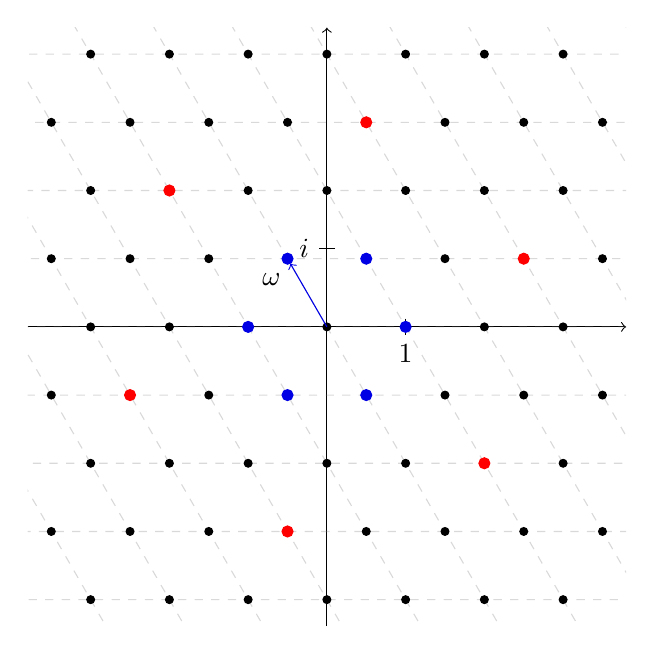
\begin{tikzpicture}
				\clip (-3.8, -3.8) rectangle (3.8, 3.8);
				\draw [->] (-3.8, 0) -- (3.8, 0);
				\draw [->] (0, -3.8) -- (0, 3.8);
				
				\draw (1,3pt) -- (1,-3pt) node [below] {$1$};
				\draw (3pt,1) -- (-3pt,1) node [left] {$i$};
				
				\pgftransformcm{1}{0}{-1/2}{1.7320501/2}{\pgfpoint{0cm}{0cm}}
				\draw[style=help lines,dashed, thin, gray, opacity=0.3] (-6,-6) grid (6,6);
				
				\foreach \x in {-5, -4, ..., 5}{
					\foreach \y in {-5, -4, ..., 5}{
						\node[draw,circle,inner sep=1pt,fill] at (\x, \y) {};
					}
				}
				
				\draw [->, black!10!blue] (0, 0) -- (0, 0.93) node [black, below left] {$\omega$};
				\node[draw,circle,inner sep=1.4pt,fill,black!10!blue] at (0, 1) {};
				\node[draw,circle,inner sep=1.4pt,fill,black!10!blue] at (0, -1) {};
				\node[draw,circle,inner sep=1.4pt,fill,black!10!blue] at (1, 0) {};
				\node[draw,circle,inner sep=1.4pt,fill,black!10!blue] at (-1, 0) {};
				\node[draw,circle,inner sep=1.4pt,fill,black!10!blue] at (1, 1) {};
				\node[draw,circle,inner sep=1.4pt,fill,black!10!blue] at (-1, -1) {};
				
				\node[draw,circle,inner sep=1.4pt,fill,red] at (3, 1) {};
				\node[draw,circle,inner sep=1.4pt,fill,red] at (-3, -1) {};
				\node[draw,circle,inner sep=1.4pt,fill,red] at (2, 3) {};
				\node[draw,circle,inner sep=1.4pt,fill,red] at (-2, -3) {};
				\node[draw,circle,inner sep=1.4pt,fill,red] at (1, -2) {};
				\node[draw,circle,inner sep=1.4pt,fill,red] at (-1, 2) {};
			\end{tikzpicture}
		}
	\end{center}
\end{example}

\begin{definition}
	Элемент $p \in K \backslash (\{0\} \cup K^*)$ называется \textit{неразложимым}, если все делители $p$ либо обратимы, либо ассоциированны с $p$.
\end{definition}

\begin{note}
	Можно эквивалентным образом определить неразложимый элемент как элемент $p \in K \backslash (\{0\} \cup K^*)$ такой, что $\forall a, b \in K: p = ab \ra a \in K^*$ или $b \in K^*$.
\end{note}

\begin{example}
	Рассмотрим $\Z[i]$ и заметим, что в $\Z[i]$ неразложимы элементы $z \in \Z[i]$ такие, что $N(z) = p$ "--- простое число, поскольку $\forall u, v \in \Z[i]: z = uv \ra N(u)N(v) = p \lra N(u) = 1$ или $N(v) = 1$. Однако существуют неразложимые элементы, норма которых не является простым числом, например, 3. Действительно, $\forall u, v \in \Z[i]: 3 = uv \ra N(u)N(v) = 9 \hm\lra N(u) = 1$ или $N(v) = 1$, поскольку в $\Z[i]$ нет элементов с нормой 3.
\end{example}

\begin{definition}
	Область целостности $K$ называется \textit{факториальным кольцом}, если для всех $x \in K \backslash \{0\}$ выполнены условия:
	\begin{enumerate}
		\item $x$ представим в виде $x = up_1\dotsm p_s$, где $u \in K^*$, $p_1, \dotsc, p_s$ "--- неразложимые (разложение $x$ \textit{существует})
		\item если $x = up_1\dotsm p_s = wq_1 \dotsm q_l$, где $u, w \in K^*$, $p_1, \dotsc, p_s, q_1, \dotsc, q_l$ "--- неразложимые, то $l = s$ и $\exists \sigma \in S_s: \forall i \in \{1, \dotsc, s\}: p_i \sim q_{\sigma(i)}$ (разложение $x$ \textit{единственно})
	\end{enumerate}
\end{definition}

\begin{example}
	Факториальными кольцами являются, например, $\Z$, $F[x]$, где $F$ "--- поле. Рассмотрим теперь область целостности $\Z[2i]$, имеющую следующий вид:
	\begin{center}
		\scalebox{0.85}{
			\begin{tikzpicture}
				\clip (-3.8, -2.8) rectangle (3.8, 2.8);
				\draw [->] (-3.8, 0) -- (3.8, 0);
				\draw [->] (0, -2.8) -- (0, 2.8);
				
				\draw (1,3pt) -- (1,-3pt) node [below] {$1$};
				\draw (3pt,1) -- (-3pt,1) node [left] {$i$};
				\pgftransformcm{1}{0}{0}{2}{\pgfpoint{0cm}{0cm}}
				\draw[style=help lines,dashed, thin, gray, opacity=0.3] (-6,-6) grid (6,6);
				
				\foreach \x in {-5, -4, ..., 5}{
					\foreach \y in {-2, -1, ..., 2}{
						\node[draw,circle,inner sep=1pt,fill] at (\x, \y) {};
					}
				}
				
				\node[draw,circle,inner sep=1.5pt,fill,black!10!blue] at (1, 0) {};
				\node[draw,circle,inner sep=1.5pt,fill,black!10!blue] at (-1, 0) {};
			\end{tikzpicture}
		}
	\end{center}
	
	Покажем, что $\Z[2i]$ не является факториальным кольцом. Аналогично случаю $\Z[i]$ можно показать, что $\Z[2i]^* = \{\pm1\}$, и элементы $2, 2i$ неразложимы. Тогда $4 = 1 \cdot 2 \cdot 2 \hm= (-1)\cdot (2i) \cdot (2i)$, но $2 \not\sim 2i$.
\end{example}

\begin{note}
	Бывают также области целостности, в которых разложения не существует. Рассмотрим $K := \{x \in \R: \exists a_0, \dotsc, a_{n - 1} \in \Z: x^n + a_{n-1}x^{n-1} + \dotsb + a_0 = 0\}$. Можно показать, что $K$ "--- действительно область целостности. Тогда $K^* = \{\pm1\}$, но неразложимых элементов в $K$ нет, поскольку $\forall a \in K \backslash (\{0\} \cup K^*): a = \sqrt{a} \cdot \sqrt{a}$, $\sqrt{a} \in K \backslash (\{0\} \cup K^*)$. Значит, разложение в $K$ существует только у элементов из $K^* = \{\pm1\}$.
\end{note}

\begin{definition}
	Элемент $p \in K \backslash (\{0\} \cup K^*)$ называется \textit{простым}, если для любых $x, y \hm\in K$ выполнено $p \mid ab \ra p \mid a$ или $p \mid b$.
\end{definition}

\begin{note}
	Легко видеть, что всякий простой элемент является неразложимым. Обратное же верно не всегда.
\end{note}

\begin{proposition}
	Если в $K$ существует разложение каждого ненулевого элемента и каждый неразложимый элемент в $K$ прост, то $K$ "--- факториальное кольцо.
\end{proposition}

\begin{proof}
	Достаточно доказать единственность разложения. Пусть $x \in K\backslash\{0\}$ и $x = up_1\dotsm p_s = wq_1\dotsm q_l$, где $u, w \in K^*$, $p_1, \dotsc, p_s, q_1, \dotsc, q_l$ "--- неразложимые, $s$ "--- наименьшее среди всех элементов с неединственным разложением. Поскольку элемент $p_1$ "--- простой, то или $p_1\mid w$, или $p_1 \mid q_1$, \dots, или $p_1 \mid q_l$. Первое невозможно, поскольку $p_1 \not\in K^*$, поэтому $p_1 \mid q_i$ для некоторого $i \in \{1, \dotsc, l\}$. Поскольку $q_i$ "--- неразложимый, то $p_1 \sim q_i$, поэтому обе части равенства можно сократить на $p_1$. Но тогда разложение элемента $up_2\dotsm p_s$ не единственно, что противоречит минимальности $s$.
\end{proof}